\begin{frame}{Overview: Workflow}
	\begin{overlayarea}{\textwidth}{.1\textheight}
	\only<1>{What the user sees:}
    \only<2>{CAD design including specification of loads and fixtures}
	\only<3>{Voxelized topology}
	\only<4>{Optimized topology}
	\only<5>{Surface extraction}
	\only<6>{Fit B-Spline surface}
	\end{overlayarea}
	\begin{overlayarea}{\textwidth}{.9\textheight}
    \begin{center}
		\begin{tikzpicture} 
        \uncover<1->{
        \node at (0,3)[inner sep=0pt](N1)
                {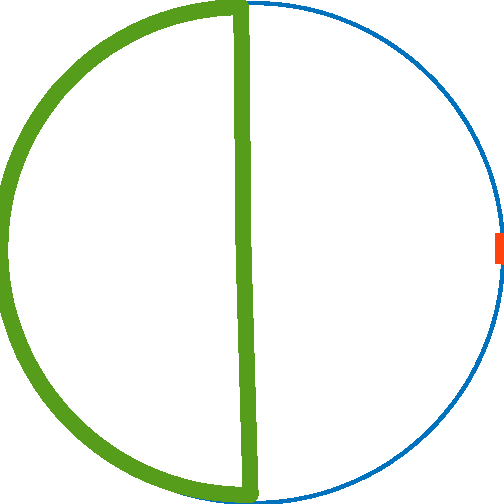
\includegraphics[width=2cm]{Pictures/1CAD_colored.pdf}};
		}
        \uncover<1->{
        \node at (0,0)[inner sep=0pt](N5)
		{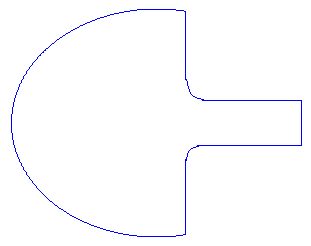
\includegraphics[width=2.2cm,height=2.2cm]{Pictures/End.png}};                        
		}        
        \uncover<1-1>{
       \draw[thick,->] (N1) -- (N5); 
		 }     
        \uncover<3->{
        \node at (4.5,3)[inner sep=0pt](N2)             
                {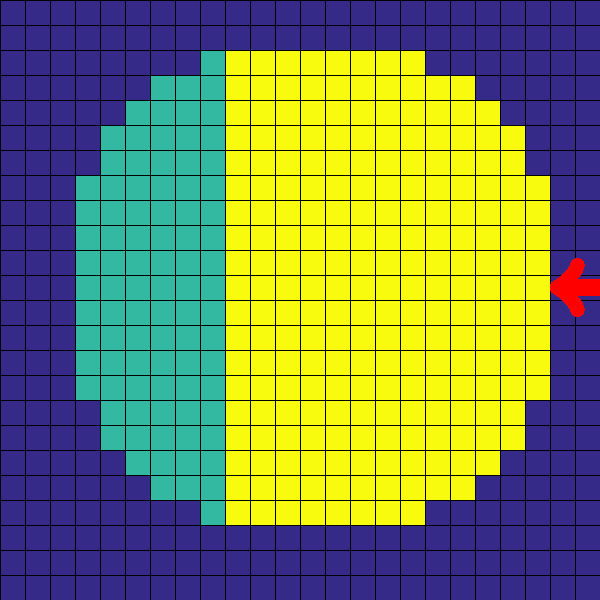
\includegraphics[width=2cm]{Pictures/4TPD.pdf}};
        \draw[thick,->] (N1) -- (N2);
        }
        \uncover<4->{
        \node at (9,1.5)[inner sep=0pt](N3) 
                {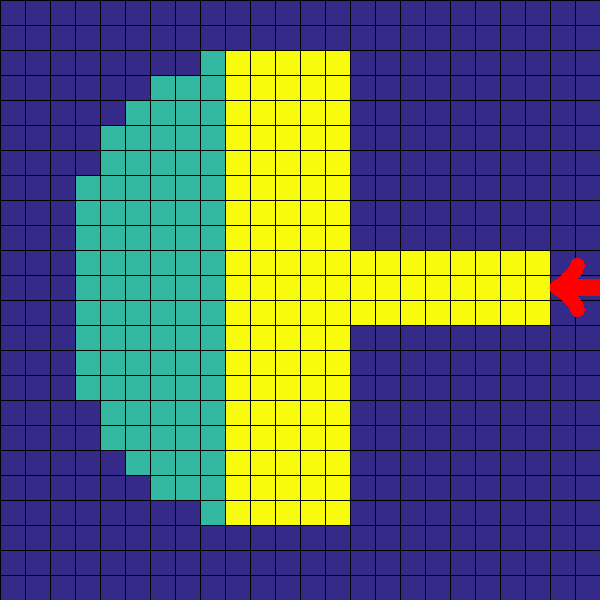
\includegraphics[width=2cm]{Pictures/5TOPOPT.pdf}};
        \draw[thick,->] (N2) -- (N3); 
        }
        \uncover<5->{
        \node at (4.5,0)[inner sep=0pt](N4)
                {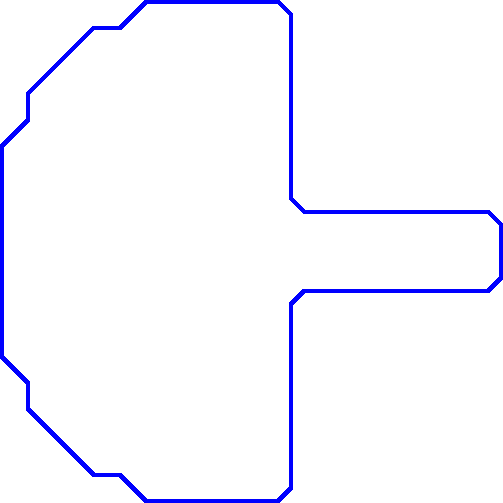
\includegraphics[width=2cm]{Pictures/7MC.pdf}};
        \draw[thick,->] (N3) -- (N4);
        }
        \uncover<6->{\draw[thick,->] (N4) -- (N5); 
        }

        \end{tikzpicture}
	\end{center}
	\end{overlayarea}

\end{frame}
